\chapter{Caching Model}
\label{chapter:caching_model}

In order to get a common understanding of caching and the terminology related to the topic, we will go through the basics of caching by describing the architecture of a web system using a cache, present a model based on a timeline that introduces the different events involved in caching and last we list criteria for evaluating a caching technique in order to choose an appropriate technique for a given use case.

\section{Caching Basics}
\label{sec:caching_basics}

In general caching is about storing the result of a computation at a where you
are able to retrieve it fast, such that it is possible to get the result fast
instead of recomputing it. This basic algorithm is illustrated on
figure~\ref{fig:basic-caching} and can be described as following:

\begin{enumerate}
  \item The result $v$ of a computation $f$ is requested.
  \item We check if $v$ is cached and is valid.
    \begin{itemize}
      \item[2a] If $v$ is cached and valid, we return $v$ and terminate.
      \item[2b] Else we compute $f$
    \end{itemize}
  \item The new value $v'$ is stored in the cache.
  \item $v'$ is returned.
\end{enumerate}

\begin{figure*}[ht!]
  \centering
  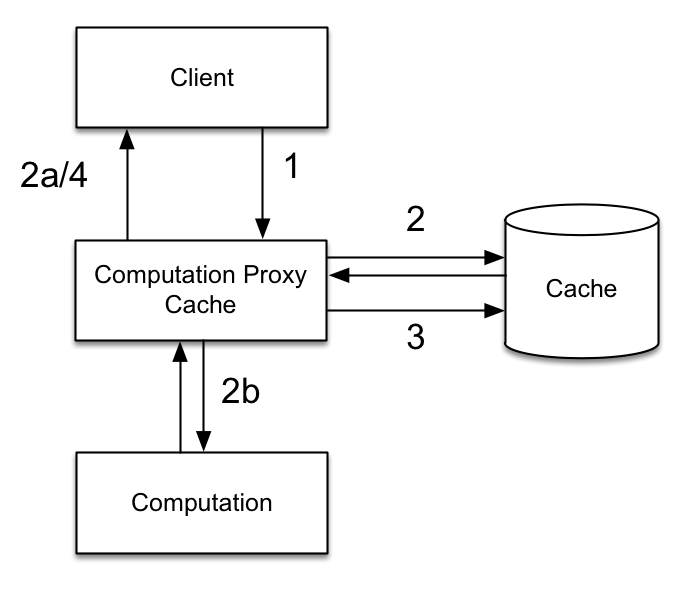
\includegraphics[width=0.5\linewidth]{figures/basic-caching-figure.png}
  \caption{The flow of basic caching}
  \label{fig:basic-caching}
\end{figure*}

If we look at the cached value from an abstract point of view, we can see it
as a \emph{result of a function} given certain \emph{inputs}. Sometimes the
inputs are data from a storage system, sometimes it's the result of an API call
to some external resource, sometimes it's global variables in the code. These
\emph{inputs} we from now on be referred to as \emph{underlying data}.

In order for the algorithm to work, we need to be sure that when we store
the cached value it has to be uniquely identified by some key such that when
we lookup the value as in step 2 of the algorithm, we always locate $v$. This
presents one of the challenges of cache management, which is in many cases
closely related to cache invalidation (one of the two hard things in computer science\footnote{At least a favorite saying of Martin Fowler and quote by Phil Karlton}).

In the algorithm cache invalidation is simply described as a \emph{check}, but
in reality this is the hard challenge of caching. The \emph{check} could be
a precomputed indicator from earlier triggers, it could be based on a key
derived from the underlying data or some timestamp. These cache invalidation
approaches will be described more in






% Introduce how caching works
% How does caching work?
%

\subsection{Architecture}
\label{subsec:architecture}

% Show the architecture of a web application with a cache
%   This figure should be used to describe architecture specific techniques

% subsection architecture end

\subsection{Timeline Model}
\label{subsec:timeline_model}

% Show the timeline model
% Introduce terminology:
%   - Value registration
%   - Invalidation
%   - Cache update
%   - Value request
% As example:
%   - Show that we when we have the given architecture, we have
%     multiple concurrent timelines running as in a distributed system
%     => We can assume that each timeline is a process

% subsection timeline_model end

% section caching_basics end

\section{Evaluating Caching Techniques}
\label{sec:evaluating_caching_techniques}

% Goals
% - What are the goals of caching:
% - We don't want the users to wait (/ performance)
% - Use less CPU

% From that desirable properties:
% - Freshness
%   - fresh is better, stale is worse
% - Consistency
%   - cached content should be as consistent with the rest of the system as possible
% - Ease of management (for the developer)
%   - The less effort (= code + thinking/complexity) to cache a given result, the better
%   - We don't want errors, when the related code is changed/extended
%     => E.g. if a new developer introduces a new data source, it should not break
%     => Or at least it should be as easy to detect these things as possible
% - Cache hit rate
%   - This depends on the amount of updates to the underlying data
%   - We can separate between:
%     - The user (have to / does not have to) wait for a given computation every time it is updated
%       => Have to: bad for cached content that is frequently updated + long running computations
%       => Not have to: great for long computations
%     -

% List how we evaluate the different caching techniques to find the right
% technique for the given use case

% - Evaluating caching technique
%   - Freshness
%   - Consistency
%   - Ease of management (invalidation)
%   - Have to wait for computation?

% section evaluating_caching_techniques end

% chapter caching_model end

